\documentclass[]{article}
\usepackage{lmodern}
\usepackage{amssymb,amsmath}
\usepackage{ifxetex,ifluatex}
\usepackage{fixltx2e} % provides \textsubscript
\ifnum 0\ifxetex 1\fi\ifluatex 1\fi=0 % if pdftex
  \usepackage[T1]{fontenc}
  \usepackage[utf8]{inputenc}
\else % if luatex or xelatex
  \ifxetex
    \usepackage{mathspec}
  \else
    \usepackage{fontspec}
  \fi
  \defaultfontfeatures{Ligatures=TeX,Scale=MatchLowercase}
\fi
% use upquote if available, for straight quotes in verbatim environments
\IfFileExists{upquote.sty}{\usepackage{upquote}}{}
% use microtype if available
\IfFileExists{microtype.sty}{%
\usepackage{microtype}
\UseMicrotypeSet[protrusion]{basicmath} % disable protrusion for tt fonts
}{}
\usepackage[margin=1in]{geometry}
\usepackage{hyperref}
\hypersetup{unicode=true,
            pdftitle={Final Writeup},
            pdfauthor={Phuc Nguyen, Ezinne Nwankwo, Frances Hung},
            pdfborder={0 0 0},
            breaklinks=true}
\urlstyle{same}  % don't use monospace font for urls
\usepackage{color}
\usepackage{fancyvrb}
\newcommand{\VerbBar}{|}
\newcommand{\VERB}{\Verb[commandchars=\\\{\}]}
\DefineVerbatimEnvironment{Highlighting}{Verbatim}{commandchars=\\\{\}}
% Add ',fontsize=\small' for more characters per line
\usepackage{framed}
\definecolor{shadecolor}{RGB}{248,248,248}
\newenvironment{Shaded}{\begin{snugshade}}{\end{snugshade}}
\newcommand{\AlertTok}[1]{\textcolor[rgb]{0.94,0.16,0.16}{#1}}
\newcommand{\AnnotationTok}[1]{\textcolor[rgb]{0.56,0.35,0.01}{\textbf{\textit{#1}}}}
\newcommand{\AttributeTok}[1]{\textcolor[rgb]{0.77,0.63,0.00}{#1}}
\newcommand{\BaseNTok}[1]{\textcolor[rgb]{0.00,0.00,0.81}{#1}}
\newcommand{\BuiltInTok}[1]{#1}
\newcommand{\CharTok}[1]{\textcolor[rgb]{0.31,0.60,0.02}{#1}}
\newcommand{\CommentTok}[1]{\textcolor[rgb]{0.56,0.35,0.01}{\textit{#1}}}
\newcommand{\CommentVarTok}[1]{\textcolor[rgb]{0.56,0.35,0.01}{\textbf{\textit{#1}}}}
\newcommand{\ConstantTok}[1]{\textcolor[rgb]{0.00,0.00,0.00}{#1}}
\newcommand{\ControlFlowTok}[1]{\textcolor[rgb]{0.13,0.29,0.53}{\textbf{#1}}}
\newcommand{\DataTypeTok}[1]{\textcolor[rgb]{0.13,0.29,0.53}{#1}}
\newcommand{\DecValTok}[1]{\textcolor[rgb]{0.00,0.00,0.81}{#1}}
\newcommand{\DocumentationTok}[1]{\textcolor[rgb]{0.56,0.35,0.01}{\textbf{\textit{#1}}}}
\newcommand{\ErrorTok}[1]{\textcolor[rgb]{0.64,0.00,0.00}{\textbf{#1}}}
\newcommand{\ExtensionTok}[1]{#1}
\newcommand{\FloatTok}[1]{\textcolor[rgb]{0.00,0.00,0.81}{#1}}
\newcommand{\FunctionTok}[1]{\textcolor[rgb]{0.00,0.00,0.00}{#1}}
\newcommand{\ImportTok}[1]{#1}
\newcommand{\InformationTok}[1]{\textcolor[rgb]{0.56,0.35,0.01}{\textbf{\textit{#1}}}}
\newcommand{\KeywordTok}[1]{\textcolor[rgb]{0.13,0.29,0.53}{\textbf{#1}}}
\newcommand{\NormalTok}[1]{#1}
\newcommand{\OperatorTok}[1]{\textcolor[rgb]{0.81,0.36,0.00}{\textbf{#1}}}
\newcommand{\OtherTok}[1]{\textcolor[rgb]{0.56,0.35,0.01}{#1}}
\newcommand{\PreprocessorTok}[1]{\textcolor[rgb]{0.56,0.35,0.01}{\textit{#1}}}
\newcommand{\RegionMarkerTok}[1]{#1}
\newcommand{\SpecialCharTok}[1]{\textcolor[rgb]{0.00,0.00,0.00}{#1}}
\newcommand{\SpecialStringTok}[1]{\textcolor[rgb]{0.31,0.60,0.02}{#1}}
\newcommand{\StringTok}[1]{\textcolor[rgb]{0.31,0.60,0.02}{#1}}
\newcommand{\VariableTok}[1]{\textcolor[rgb]{0.00,0.00,0.00}{#1}}
\newcommand{\VerbatimStringTok}[1]{\textcolor[rgb]{0.31,0.60,0.02}{#1}}
\newcommand{\WarningTok}[1]{\textcolor[rgb]{0.56,0.35,0.01}{\textbf{\textit{#1}}}}
\usepackage{graphicx,grffile}
\makeatletter
\def\maxwidth{\ifdim\Gin@nat@width>\linewidth\linewidth\else\Gin@nat@width\fi}
\def\maxheight{\ifdim\Gin@nat@height>\textheight\textheight\else\Gin@nat@height\fi}
\makeatother
% Scale images if necessary, so that they will not overflow the page
% margins by default, and it is still possible to overwrite the defaults
% using explicit options in \includegraphics[width, height, ...]{}
\setkeys{Gin}{width=\maxwidth,height=\maxheight,keepaspectratio}
\IfFileExists{parskip.sty}{%
\usepackage{parskip}
}{% else
\setlength{\parindent}{0pt}
\setlength{\parskip}{6pt plus 2pt minus 1pt}
}
\setlength{\emergencystretch}{3em}  % prevent overfull lines
\providecommand{\tightlist}{%
  \setlength{\itemsep}{0pt}\setlength{\parskip}{0pt}}
\setcounter{secnumdepth}{0}
% Redefines (sub)paragraphs to behave more like sections
\ifx\paragraph\undefined\else
\let\oldparagraph\paragraph
\renewcommand{\paragraph}[1]{\oldparagraph{#1}\mbox{}}
\fi
\ifx\subparagraph\undefined\else
\let\oldsubparagraph\subparagraph
\renewcommand{\subparagraph}[1]{\oldsubparagraph{#1}\mbox{}}
\fi

%%% Use protect on footnotes to avoid problems with footnotes in titles
\let\rmarkdownfootnote\footnote%
\def\footnote{\protect\rmarkdownfootnote}

%%% Change title format to be more compact
\usepackage{titling}

% Create subtitle command for use in maketitle
\providecommand{\subtitle}[1]{
  \posttitle{
    \begin{center}\large#1\end{center}
    }
}

\setlength{\droptitle}{-2em}

  \title{Final Writeup}
    \pretitle{\vspace{\droptitle}\centering\huge}
  \posttitle{\par}
    \author{Phuc Nguyen, Ezinne Nwankwo, Frances Hung}
    \preauthor{\centering\large\emph}
  \postauthor{\par}
      \predate{\centering\large\emph}
  \postdate{\par}
    \date{2/19/2020}


\begin{document}
\maketitle

\begin{abstract}
In this paper, we study the factors that influence college drinking behavior and its effects on other harmful behaviors, in particular sexual assault. We answer three main questions of interest: first to understand the factors that influence college drinking behavior, second to access if current school policies and methods of spreading resources around drinking had any influence on college drinking behavior, and third to understand the relationship between college drinking behavior and sexual assault while accounting for other confounding factors (i.e. family drinking behaviour, etc.). Through the use of mediatian analysis and structural equation models, we are able to isolate the direct effect of other factors on sexual assault and their indirect effect through college drinking behavior. We conclude that high school drinking behavior had the largest effects, both directly indirectly, on college drinking behavior and on incidences of sexual assault. 
\end{abstract}

\hypertarget{introduction}{%
\subsection{Introduction}\label{introduction}}

Drinking in college is almost like a right of passage. And while
policies around college campus seem to vary in terms of strictness, most
of them have much more relaxed policies than bars and clubs. Instead
what schools care about are the dangerous activities that drinking leads
to, such as sexual assault and drunk driving. For this study, we focus
on understanding sexual assault, as it is a very pervasive and pertinent
issue on campuses everywhere.

We are interested in studying three questions: (i.) the factors that
influence college drinking behavior (ii.) how certain school policies
influence drinking behavior (iii.) and then how those behaviors lead to
other more harmful behaviors in the hopes that we can help colleges try
to prevent some of these more serious issues.

\hypertarget{data-cleaning}{%
\subsection{Data Cleaning}\label{data-cleaning}}

Due to the structure of the survey (students skip certain questions
based on their answers), there are a lot of missing values induced in
the data for certain variables. We impute zero values for NAs if the
variables are ordinal and if NAs are naturally lowest in the ordinal
structure. Otherwise, we create indicator variables for whether a person
answered NA or not for each variable in question. We additionally drop
true missing values.

\hypertarget{exploratory-data-analysis}{%
\subsection{Exploratory Data Analysis}\label{exploratory-data-analysis}}

We look at drinking patterns casually by visualizing some survey
question responses from Section C, which is about drinking patterns in
college. By looking at histograms, we can see that drinking at
off-campus parties and bars results in the highest number of drinks
taken. The reasons students cited as most important for drinking were
getting drunk and as a reward. This suggests that drinking location and
social groups may be important predictors of drinking behavior.

For our dependent variable measuring drinking behavior, we choose to use
\(\texttt{drinkcat}\), a variable created by researchers which
classifies drinking behavior into four ordinal risk categories. The
sexual assault index variable draws from three questions in the survey:
D5\_H (unwanted sexual advance), D5\_I (date rape/sexual assault), E15
(intoxicated, unable to consent).

\hypertarget{methods}{%
\subsection{Methods}\label{methods}}

We use Structural Equation Modeling (SEM) for modeling causal
relationships between information collected via the survey and our
dependent variables \(\texttt{drinkcat}\) and
\(\texttt{sexassault_ind}\). The SEM package we use in R,
\(\texttt{lavaan}\), uses partial least squares regression to find a
linear model relating the independent and dependent variables through
latent factors. We standardize all of the variables we use in order to
make our coefficients interpretable and comparable in the final model.

We create the following latent factors from existing survey question
variables (Fig. \ref{fig:latent-vars}). Since these factors must be
correlated, interpretable, and continuous (due to our use of the
\(\texttt{lavaan}\) package), we ensure that the survey question
variables included in each factor are uniformly ordinal in an
interpretable way. Our two factors related to students' pre-college
lives are Family Education/Drinking (G14-17) and High School Drinking
Behavior (G9-11). The external-policy related factors are College
Alcohol Policy (B1, B2, B9), College Alcohol Education (B7, B8), and
City Alcohol Policy (B11-13). The rest of the latent factors have to do
with students' college experiences and opinions: Academic Wellbeing (F1,
F4), Personal Wellbeing (F6), Support for Stricter Policies (D3),
Opinions on \# Appropriate Drinks (D1), Time Spent on Activities (F5),
and General Interests for College Experience (split into activities
involving and not involving partying/Greek life, A10).

In order to understand the relationships between drinking behaviors and
sexual assault, we fit another latent factor model with mediation on the
indicator of being a victim of sexual assault given family
education/drinking background, high school, college drinking behavior,
and participations in parties. Mediation analysis allows us to estimate
how much of the association between a risk factor, such as participation
in parties, and the risk of sexual assault is mediated by the victim's
drinking behavior.

\hypertarget{results}{%
\subsection{Results}\label{results}}

\hypertarget{drinking-behavior}{%
\subsubsection{Drinking Behavior}\label{drinking-behavior}}

Table \ref{fig:tab-coefs} shows the estimates and 95\% confidence
intervals for the coefficents of latent variables in the drinking
behavior model. We accept the model as its RMSEA 95\% CI of
\([0.053, 0.054]\) is around the conventional threshold of 0.05 for a
good fit (CITE). Since the survey answers generally did not have
physical units, we standardized the variables to compare the size of the
estimated coefficients. The dependent variable, i.e.~the rating of
levels of drinking, also does not have physical units. Thus, we will
interpret these coefficents in terms of the relative magnitude and
direction of their association with heavier drinking. High school
drinking history is most correlated with more drinking in college. The
latent factor Parties summarizing the importance of fraternity/sorority,
parties and athletics to students (A10), with a lower value
corresponding to more importance, has the second largest association. In
other words, students who participate more in the mentioned activities
tend to drink more. The variable Communities measures the importance of
other activities such as volunteering, religion, arts, activism and
academic (A10), has the third largest association. Students who care
less about these activities tend to drink more. Fourthly, students who
perceive a larger number of drink appropriate tend to drink more. Other
latent variables with significant but smaller associations with heavier
drinking in college include Personal Wellbeing, Family
Education/Drinking and Support for More Lenient Policy. Specifically,
students who are generally more happy, whose families approve of
drinking, or who support more lenient drinking policies on campus tend
to drink more. There is not enough evidence to establish a relationship
between stricter college drinking policy and drinking behaviors. We find
a small association between more exposure to alcohol/drinking education
and heavier drinkers. We hypothesize that students who already have
drinking problems or schools with more prevalent drinking culture might
consequently have more educational programs on the issue.

\hypertarget{risk-of-sexual-assault}{%
\subsubsection{Risk of Sexual Assault}\label{risk-of-sexual-assault}}

\hypertarget{sensitivity-analysis}{%
\subsection{Sensitivity Analysis}\label{sensitivity-analysis}}

We can compare our SEM model for college drinking severity to an elastic
net model created using the \(\texttt{glmnet}\) package. Both of these
models carry out dimension reduction, so it is interesting and
reassuring to note that the results of both seem to corraborate one
another. From the elastic net model, the most important predictors for
heavy drinkers are A10\_F(parties, -), B6\_D (times they were part of
drinking group which was asked to be quieter/less disruptive, +), D1\_B
(opinion on appropriate amount for off-campus bar drinking, +), D9\_B
(percentage of friends who are binge drinkers, +), and G11 (HS number of
binges, +). This supports the results of our latent factor model, which
finds strong correlations of college drinking with drinking attitudes,
emphasis on partying, and high school drinking.

\hypertarget{references}{%
\subsection{References}\label{references}}

\url{https://www.ncbi.nlm.nih.gov/pmc/articles/PMC2819368/}

\url{http://lavaan.ugent.be/index.html}

An Introduction to Structural Equation Modeling. J.J. Hox. University of
Amsterdam/Utrecht University

\hypertarget{figures}{%
\subsection{Figures}\label{figures}}

\hypertarget{r-num-drinks-eda-echofalse-evaltrueout.width-500px-fig.aligncenter-fig.caplabelfignum-drinks-edafigure-shows-latent-factors-ovals-in-the-sem-for-drinking-behaviors.-squares-show-summary-of-actual-questions-in-the-survey.-knitrinclude_graphicsplotsnum_drink_plot.png}{%
\section{\texorpdfstring{\texttt{\{r\ num-drinks-eda,\ echo=FALSE,\ eval=TRUE,out.width\ =\ "500px",\ fig.align="center",\ fig.cap="\textbackslash{}\textbackslash{}label\{fig:num-drinks-eda\}Figure\ shows\ latent\ factors\ (ovals)\ in\ the\ SEM\ for\ drinking\ behaviors.\ Squares\ show\ summary\ of\ actual\ questions\ in\ the\ survey."\}\ \#\ knitr::include\_graphics("plots/num\_drink\_plot.png")\ \#}}{\{r num-drinks-eda, echo=FALSE, eval=TRUE,out.width = "500px", fig.align="center", fig.cap="\textbackslash{}\textbackslash{}label\{fig:num-drinks-eda\}Figure shows latent factors (ovals) in the SEM for drinking behaviors. Squares show summary of actual questions in the survey."\} \# knitr::include\_graphics("plots/num\_drink\_plot.png") \#}}\label{r-num-drinks-eda-echofalse-evaltrueout.width-500px-fig.aligncenter-fig.caplabelfignum-drinks-edafigure-shows-latent-factors-ovals-in-the-sem-for-drinking-behaviors.-squares-show-summary-of-actual-questions-in-the-survey.-knitrinclude_graphicsplotsnum_drink_plot.png}}

\hypertarget{r-reasons-eda-echofalse-evaltrueout.width-500px-fig.aligncenter-fig.caplabelfiglatent-varsfigure-shows-latent-factors-ovals-in-the-sem-for-drinking-behaviors.-squares-show-summary-of-actual-questions-in-the-survey.-knitrinclude_graphicsplotsreasons_plot.png}{%
\section{\texorpdfstring{\texttt{\{r\ reasons-eda,\ echo=FALSE,\ eval=TRUE,out.width\ =\ "500px",\ fig.align="center",\ fig.cap="\textbackslash{}\textbackslash{}label\{fig:latent-vars\}Figure\ shows\ latent\ factors\ (ovals)\ in\ the\ SEM\ for\ drinking\ behaviors.\ Squares\ show\ summary\ of\ actual\ questions\ in\ the\ survey."\}\ \#\ knitr::include\_graphics("plots/reasons\_plot.png")\ \#}}{\{r reasons-eda, echo=FALSE, eval=TRUE,out.width = "500px", fig.align="center", fig.cap="\textbackslash{}\textbackslash{}label\{fig:latent-vars\}Figure shows latent factors (ovals) in the SEM for drinking behaviors. Squares show summary of actual questions in the survey."\} \# knitr::include\_graphics("plots/reasons\_plot.png") \#}}\label{r-reasons-eda-echofalse-evaltrueout.width-500px-fig.aligncenter-fig.caplabelfiglatent-varsfigure-shows-latent-factors-ovals-in-the-sem-for-drinking-behaviors.-squares-show-summary-of-actual-questions-in-the-survey.-knitrinclude_graphicsplotsreasons_plot.png}}

\begin{figure}

{\centering 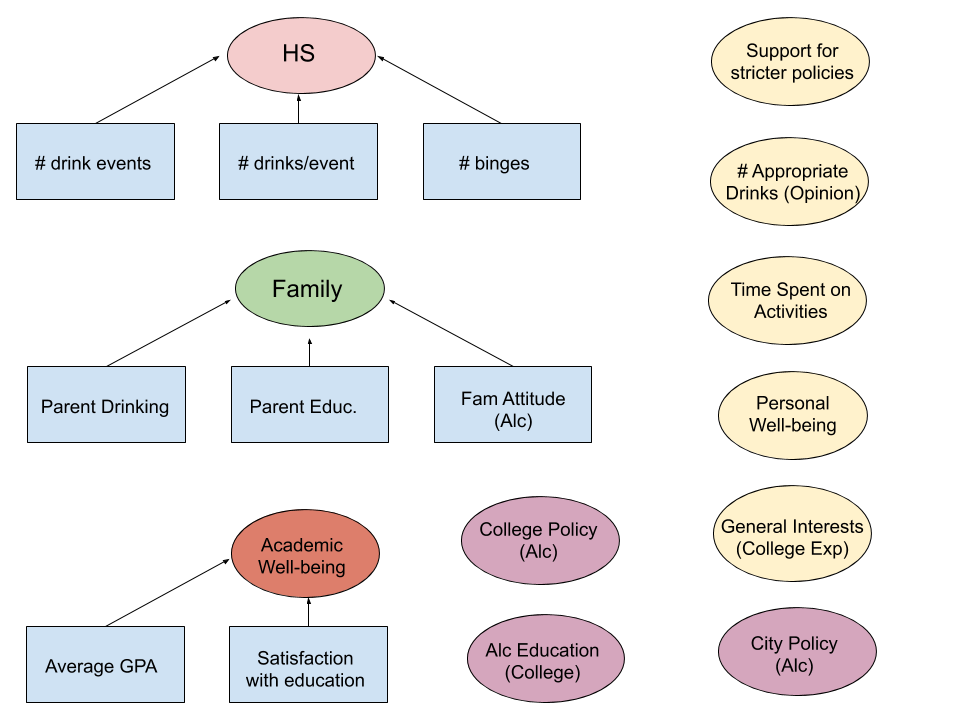
\includegraphics[width=500px]{plots/latent_vars} 

}

\caption{\label{fig:latent-vars}Figure shows latent factors (ovals) in the SEM for drinking behaviors. Squares show summary of actual questions in the survey.}\label{fig:latent-vars}
\end{figure}

\hypertarget{appendix}{%
\subsection{Appendix}\label{appendix}}

\hypertarget{data-cleaning-1}{%
\subsection{Data Cleaning}\label{data-cleaning-1}}

\hypertarget{reading-in-data}{%
\subsubsection{Reading In Data}\label{reading-in-data}}

Split file by number of columns for each variable in Record\_layout.txt
file. Spaces are missing values.

\begin{Shaded}
\begin{Highlighting}[]
\NormalTok{read_cas <-}\StringTok{ }\ControlFlowTok{function}\NormalTok{(folder, file, recordfile) \{}
\NormalTok{  skip <-}\StringTok{ }\KeywordTok{grep}\NormalTok{(}\StringTok{"--------"}\NormalTok{, }\KeywordTok{readLines}\NormalTok{(}\KeywordTok{unz}\NormalTok{(folder, recordfile)))}
\NormalTok{  record_layout <-}\StringTok{ }\KeywordTok{read.table}\NormalTok{(}\KeywordTok{unz}\NormalTok{(folder, recordfile), }
                            \DataTypeTok{fill =} \OtherTok{TRUE}\NormalTok{, }\DataTypeTok{skip =}\NormalTok{ skip, }\DataTypeTok{header =} \OtherTok{FALSE}\NormalTok{)}
  \KeywordTok{colnames}\NormalTok{(record_layout) <-}\StringTok{ }\KeywordTok{c}\NormalTok{(}\StringTok{"variable_name"}\NormalTok{, }\StringTok{"start_col"}\NormalTok{, }\StringTok{"end_col"}\NormalTok{, }\StringTok{"type"}\NormalTok{)}
\NormalTok{  record_layout <-}\StringTok{ }\NormalTok{record_layout }\OperatorTok\StringTok{ }\KeywordTok{filter}\NormalTok{(}\OperatorTok{!}\KeywordTok{is.na}\NormalTok{(end_col))}
\NormalTok{  widths <-}\StringTok{ }\KeywordTok{as.numeric}\NormalTok{(}\KeywordTok{as.character}\NormalTok{(record_layout}\OperatorTok{$}\NormalTok{end_col)) }\OperatorTok{-}\StringTok{ }\KeywordTok{as.numeric}\NormalTok{(}\KeywordTok{as.character}\NormalTok{(record_layout}\OperatorTok{$}\NormalTok{start_col)) }\OperatorTok{+}\StringTok{ }\DecValTok{1}
\NormalTok{  cas <-}\StringTok{ }\KeywordTok{read.fwf}\NormalTok{(}\KeywordTok{unz}\NormalTok{(folder, file), }\DataTypeTok{widths =}\NormalTok{ widths, }\DataTypeTok{header    =} \OtherTok{FALSE}\NormalTok{,}
                  \DataTypeTok{col.names =}\NormalTok{ record_layout}\OperatorTok{$}\NormalTok{variable_name)}
  \KeywordTok{return}\NormalTok{(cas)}
\NormalTok{\}}
\NormalTok{cas97 <-}\StringTok{ }\KeywordTok{read_cas}\NormalTok{(}\DataTypeTok{folder =} \StringTok{"Harvard_CAS_1997.zip"}\NormalTok{, }
                  \DataTypeTok{file =} \StringTok{"Harvard_CAS_1997/DS0001/03163-0001-Data.txt"}\NormalTok{,}
                  \DataTypeTok{recordfile =} \StringTok{"Harvard_CAS_1997/DS0001/03163-0001-Record_layout.txt"}\NormalTok{)}
\end{Highlighting}
\end{Shaded}

\begin{Shaded}
\begin{Highlighting}[]
\NormalTok{summary_na<-}\ControlFlowTok{function}\NormalTok{(df) \{}
\NormalTok{  na_count <-}\StringTok{ }\KeywordTok{colSums}\NormalTok{(}\KeywordTok{apply}\NormalTok{(df, }\DecValTok{2}\NormalTok{, is.na))}
  \KeywordTok{data.frame}\NormalTok{(}\DataTypeTok{name =} \KeywordTok{colnames}\NormalTok{(df), }\DataTypeTok{na_pct =}\NormalTok{ na_count}\OperatorTok{/}\KeywordTok{nrow}\NormalTok{(df)) }\OperatorTok\StringTok{ }\KeywordTok{arrange}\NormalTok{(}\KeywordTok{desc}\NormalTok{(na_pct))}
\NormalTok{\}}
\end{Highlighting}
\end{Shaded}

The survey asks students to skip some questions on purpose. We manually
go through the survey to impute these values and drop remaining missing
entries.

\hypertarget{section-a}{%
\paragraph{Section A}\label{section-a}}

\begin{Shaded}
\begin{Highlighting}[]
\CommentTok{# See which vars have lots of NA's}
\NormalTok{cas97 }\OperatorTok\StringTok{ }
\StringTok{  }\NormalTok{dplyr}\OperatorTok{::}\KeywordTok{select}\NormalTok{(}\KeywordTok{which}\NormalTok{(}\KeywordTok{grepl}\NormalTok{(}\StringTok{"^A"}\NormalTok{, }\KeywordTok{colnames}\NormalTok{(.)))) }\OperatorTok
\StringTok{  }\KeywordTok{summary_na}\NormalTok{()}

\CommentTok{# Fill in NA's that mean 0}
\NormalTok{cas97 <-}\StringTok{ }\NormalTok{cas97 }\OperatorTok
\StringTok{  }\KeywordTok{mutate}\NormalTok{(}\DataTypeTok{A8_answered =}\NormalTok{ cas97 }\OperatorTok
\StringTok{                        }\NormalTok{dplyr}\OperatorTok{::}\KeywordTok{select}\NormalTok{(}\KeywordTok{which}\NormalTok{(}\KeywordTok{grepl}\NormalTok{(}\StringTok{"^A8_"}\NormalTok{, }\KeywordTok{colnames}\NormalTok{(.)))) }\OperatorTok
\StringTok{                        }\KeywordTok{rowSums}\NormalTok{(}\DataTypeTok{na.rm =} \OtherTok{TRUE}\NormalTok{)) }\OperatorTok
\StringTok{  }\KeywordTok{mutate}\NormalTok{(}\DataTypeTok{A8_1 =} \KeywordTok{ifelse}\NormalTok{(}\KeywordTok{is.na}\NormalTok{(A8_}\DecValTok{1}\NormalTok{) }\OperatorTok{&}\StringTok{ }\NormalTok{A8_answered }\OperatorTok{>}\StringTok{ }\DecValTok{0}\NormalTok{, }\DecValTok{0}\NormalTok{, A8_}\DecValTok{1}\NormalTok{),}
         \DataTypeTok{A8_2 =} \KeywordTok{ifelse}\NormalTok{(}\KeywordTok{is.na}\NormalTok{(A8_}\DecValTok{2}\NormalTok{) }\OperatorTok{&}\StringTok{ }\NormalTok{A8_answered }\OperatorTok{>}\StringTok{ }\DecValTok{0}\NormalTok{, }\DecValTok{0}\NormalTok{, A8_}\DecValTok{2}\NormalTok{),}
         \DataTypeTok{A8_3 =} \KeywordTok{ifelse}\NormalTok{(}\KeywordTok{is.na}\NormalTok{(A8_}\DecValTok{3}\NormalTok{) }\OperatorTok{&}\StringTok{ }\NormalTok{A8_answered }\OperatorTok{>}\StringTok{ }\DecValTok{0}\NormalTok{, }\DecValTok{0}\NormalTok{, A8_}\DecValTok{3}\NormalTok{),}
         \DataTypeTok{A8_4 =} \KeywordTok{ifelse}\NormalTok{(}\KeywordTok{is.na}\NormalTok{(A8_}\DecValTok{4}\NormalTok{) }\OperatorTok{&}\StringTok{ }\NormalTok{A8_answered }\OperatorTok{>}\StringTok{ }\DecValTok{0}\NormalTok{, }\DecValTok{0}\NormalTok{, A8_}\DecValTok{4}\NormalTok{)) }\OperatorTok
\StringTok{  }\CommentTok{# A6 should be dummified}
\StringTok{  }\KeywordTok{mutate}\NormalTok{(}\DataTypeTok{ones =} \DecValTok{1}\NormalTok{) }\OperatorTok
\StringTok{  }\NormalTok{tidyr}\OperatorTok{::}\KeywordTok{pivot_wider}\NormalTok{(}\DataTypeTok{names_from =}\NormalTok{ A6, }
                     \DataTypeTok{values_from =}\NormalTok{ ones, }
                     \DataTypeTok{values_fill =} \KeywordTok{list}\NormalTok{(}\DataTypeTok{ones =} \DecValTok{0}\NormalTok{), }
                     \DataTypeTok{names_prefix =} \StringTok{"A6_"}\NormalTok{) }\OperatorTok
\StringTok{  }\CommentTok{# Some NA in A7 means student lived off campus}
\StringTok{  }\KeywordTok{mutate}\NormalTok{(}\DataTypeTok{A7 =} \KeywordTok{ifelse}\NormalTok{(}\KeywordTok{is.na}\NormalTok{(A7) }\OperatorTok{&}\StringTok{ }\NormalTok{A6_}\DecValTok{5} \OperatorTok{==}\StringTok{ }\DecValTok{1}\NormalTok{, }\DecValTok{0}\NormalTok{, A7)) }\OperatorTok
\StringTok{  }\CommentTok{# Drop A4, A5 that are transfer questions, otherwise have to dummify}
\StringTok{  }\NormalTok{dplyr}\OperatorTok{::}\KeywordTok{select}\NormalTok{(}\OperatorTok{-}\NormalTok{A4, }\OperatorTok{-}\NormalTok{A5, }\OperatorTok{-}\NormalTok{A8_answered, }\OperatorTok{-}\NormalTok{A8)}

\CommentTok{# How many complete cases left?}
\NormalTok{cas97 }\OperatorTok
\StringTok{  }\NormalTok{dplyr}\OperatorTok{::}\KeywordTok{select}\NormalTok{(}\KeywordTok{which}\NormalTok{(}\KeywordTok{grepl}\NormalTok{(}\StringTok{"^A"}\NormalTok{, }\KeywordTok{colnames}\NormalTok{(.)))) }\OperatorTok
\StringTok{  }\KeywordTok{filter}\NormalTok{(}\KeywordTok{complete.cases}\NormalTok{(.)) }\OperatorTok
\StringTok{  }\KeywordTok{nrow}\NormalTok{()}
\end{Highlighting}
\end{Shaded}

\hypertarget{section-b}{%
\paragraph{Section B}\label{section-b}}

No skipped questions

For B10, an indicator is an option, fill in zero for than NA

\begin{Shaded}
\begin{Highlighting}[]
\CommentTok{# Which columns in this section have lots of NA?}
\NormalTok{cas97 }\OperatorTok\StringTok{ }
\StringTok{  }\NormalTok{dplyr}\OperatorTok{::}\KeywordTok{select}\NormalTok{(}\KeywordTok{which}\NormalTok{(}\KeywordTok{grepl}\NormalTok{(}\StringTok{"^B"}\NormalTok{, }\KeywordTok{colnames}\NormalTok{(.)))) }\OperatorTok
\StringTok{  }\KeywordTok{summary_na}\NormalTok{()}

\CommentTok{# Fill in NA that actually means 0}
\NormalTok{cas97 <-}\StringTok{ }\NormalTok{cas97 }\OperatorTok
\StringTok{  }\KeywordTok{mutate}\NormalTok{(}\DataTypeTok{B10_answered =}\NormalTok{ cas97 }\OperatorTok
\StringTok{                        }\NormalTok{dplyr}\OperatorTok{::}\KeywordTok{select}\NormalTok{(}\KeywordTok{which}\NormalTok{(}\KeywordTok{grepl}\NormalTok{(}\StringTok{"^B10_"}\NormalTok{, }\KeywordTok{colnames}\NormalTok{(.)))) }\OperatorTok
\StringTok{                        }\KeywordTok{rowSums}\NormalTok{(}\DataTypeTok{na.rm =} \OtherTok{TRUE}\NormalTok{)) }\OperatorTok
\StringTok{  }\KeywordTok{mutate}\NormalTok{(}\DataTypeTok{B10_1 =} \KeywordTok{ifelse}\NormalTok{(}\KeywordTok{is.na}\NormalTok{(B10_}\DecValTok{1}\NormalTok{) }\OperatorTok{&}\StringTok{ }\NormalTok{B10_answered }\OperatorTok{>}\StringTok{ }\DecValTok{0}\NormalTok{, }\DecValTok{0}\NormalTok{, B10_}\DecValTok{1}\NormalTok{),}
         \DataTypeTok{B10_2 =} \KeywordTok{ifelse}\NormalTok{(}\KeywordTok{is.na}\NormalTok{(B10_}\DecValTok{2}\NormalTok{) }\OperatorTok{&}\StringTok{ }\NormalTok{B10_answered }\OperatorTok{>}\StringTok{ }\DecValTok{0}\NormalTok{, }\DecValTok{0}\NormalTok{, B10_}\DecValTok{2}\NormalTok{),}
         \DataTypeTok{B10_3 =} \KeywordTok{ifelse}\NormalTok{(}\KeywordTok{is.na}\NormalTok{(B10_}\DecValTok{3}\NormalTok{) }\OperatorTok{&}\StringTok{ }\NormalTok{B10_answered }\OperatorTok{>}\StringTok{ }\DecValTok{0}\NormalTok{, }\DecValTok{0}\NormalTok{, B10_}\DecValTok{3}\NormalTok{),}
         \DataTypeTok{B10_4 =} \KeywordTok{ifelse}\NormalTok{(}\KeywordTok{is.na}\NormalTok{(B10_}\DecValTok{4}\NormalTok{) }\OperatorTok{&}\StringTok{ }\NormalTok{B10_answered }\OperatorTok{>}\StringTok{ }\DecValTok{0}\NormalTok{, }\DecValTok{0}\NormalTok{, B10_}\DecValTok{4}\NormalTok{),}
         \DataTypeTok{B10_5 =} \KeywordTok{ifelse}\NormalTok{(}\KeywordTok{is.na}\NormalTok{(B10_}\DecValTok{5}\NormalTok{) }\OperatorTok{&}\StringTok{ }\NormalTok{B10_answered }\OperatorTok{>}\StringTok{ }\DecValTok{0}\NormalTok{, }\DecValTok{0}\NormalTok{, B10_}\DecValTok{5}\NormalTok{),}
         \DataTypeTok{B10_6 =} \KeywordTok{ifelse}\NormalTok{(}\KeywordTok{is.na}\NormalTok{(B10_}\DecValTok{6}\NormalTok{) }\OperatorTok{&}\StringTok{ }\NormalTok{B10_answered }\OperatorTok{>}\StringTok{ }\DecValTok{0}\NormalTok{, }\DecValTok{0}\NormalTok{, B10_}\DecValTok{6}\NormalTok{),}
         \DataTypeTok{B10_7 =} \KeywordTok{ifelse}\NormalTok{(}\KeywordTok{is.na}\NormalTok{(B10_}\DecValTok{7}\NormalTok{) }\OperatorTok{&}\StringTok{ }\NormalTok{B10_answered }\OperatorTok{>}\StringTok{ }\DecValTok{0}\NormalTok{, }\DecValTok{0}\NormalTok{, B10_}\DecValTok{7}\NormalTok{),}
         \DataTypeTok{B10_8 =} \KeywordTok{ifelse}\NormalTok{(}\KeywordTok{is.na}\NormalTok{(B10_}\DecValTok{8}\NormalTok{) }\OperatorTok{&}\StringTok{ }\NormalTok{B10_answered }\OperatorTok{>}\StringTok{ }\DecValTok{0}\NormalTok{, }\DecValTok{0}\NormalTok{, B10_}\DecValTok{8}\NormalTok{)) }\OperatorTok
\StringTok{  }\NormalTok{dplyr}\OperatorTok{::}\KeywordTok{select}\NormalTok{(}\OperatorTok{-}\NormalTok{B10_answered)}

\CommentTok{# How many complete cases left?}
\NormalTok{cas97 }\OperatorTok
\StringTok{  }\NormalTok{dplyr}\OperatorTok{::}\KeywordTok{select}\NormalTok{(}\KeywordTok{which}\NormalTok{(}\KeywordTok{grepl}\NormalTok{(}\StringTok{"^B"}\NormalTok{, }\KeywordTok{colnames}\NormalTok{(.)))) }\OperatorTok
\StringTok{  }\KeywordTok{filter}\NormalTok{(}\KeywordTok{complete.cases}\NormalTok{(.)) }\OperatorTok
\StringTok{  }\KeywordTok{nrow}\NormalTok{()}
\end{Highlighting}
\end{Shaded}

\hypertarget{section-c}{%
\paragraph{Section C}\label{section-c}}

\hypertarget{section-d}{%
\paragraph{Section D}\label{section-d}}

\begin{Shaded}
\begin{Highlighting}[]
\CommentTok{# Which columns in this section have lots of NA?}
\NormalTok{cas97 }\OperatorTok\StringTok{ }
\StringTok{  }\NormalTok{dplyr}\OperatorTok{::}\KeywordTok{select}\NormalTok{(}\KeywordTok{which}\NormalTok{(}\KeywordTok{grepl}\NormalTok{(}\StringTok{"^D}\CharTok{\textbackslash{}\textbackslash{}}\StringTok{d"}\NormalTok{, }\KeywordTok{colnames}\NormalTok{(.)))) }\OperatorTok
\StringTok{  }\KeywordTok{summary_na}\NormalTok{()}

\NormalTok{cas97 <-}\StringTok{ }\NormalTok{cas97 }\OperatorTok
\StringTok{  }\NormalTok{dplyr}\OperatorTok{::}\KeywordTok{select}\NormalTok{(}\OperatorTok{-}\NormalTok{D7_}\DecValTok{1}\NormalTok{, }\OperatorTok{-}\NormalTok{D7_}\DecValTok{2}\NormalTok{, }\OperatorTok{-}\NormalTok{D7_}\DecValTok{3}\NormalTok{, }\OperatorTok{-}\NormalTok{D7_}\DecValTok{4}\NormalTok{)}

\CommentTok{# How many complete cases left?}
\NormalTok{cas97 }\OperatorTok
\StringTok{  }\NormalTok{dplyr}\OperatorTok{::}\KeywordTok{select}\NormalTok{(}\KeywordTok{which}\NormalTok{(}\KeywordTok{grepl}\NormalTok{(}\StringTok{"^D}\CharTok{\textbackslash{}\textbackslash{}}\StringTok{d"}\NormalTok{, }\KeywordTok{colnames}\NormalTok{(.)))) }\OperatorTok
\StringTok{  }\KeywordTok{filter}\NormalTok{(}\KeywordTok{complete.cases}\NormalTok{(.)) }\OperatorTok
\StringTok{  }\KeywordTok{nrow}\NormalTok{()}
\end{Highlighting}
\end{Shaded}

\hypertarget{section-e}{%
\paragraph{Section E}\label{section-e}}

Possible groups to consider: Female vs Male, Younger vs Older than 21
years old

\begin{Shaded}
\begin{Highlighting}[]
\CommentTok{# Which columns in this section have lots of NA?}
\NormalTok{cas97 }\OperatorTok\StringTok{ }
\StringTok{  }\NormalTok{dplyr}\OperatorTok{::}\KeywordTok{select}\NormalTok{(}\KeywordTok{which}\NormalTok{(}\KeywordTok{grepl}\NormalTok{(}\StringTok{"^E}\CharTok{\textbackslash{}\textbackslash{}}\StringTok{d"}\NormalTok{, }\KeywordTok{colnames}\NormalTok{(.)))) }\OperatorTok
\StringTok{  }\KeywordTok{summary_na}\NormalTok{()}

\NormalTok{cas97 <-}\StringTok{ }\NormalTok{cas97 }\OperatorTok
\StringTok{  }\CommentTok{# Fill NA resulted from dummifying vars E23}
\StringTok{  }\KeywordTok{mutate}\NormalTok{(}\DataTypeTok{E23_answered =}\NormalTok{ cas97 }\OperatorTok
\StringTok{                        }\NormalTok{dplyr}\OperatorTok{::}\KeywordTok{select}\NormalTok{(}\KeywordTok{which}\NormalTok{(}\KeywordTok{grepl}\NormalTok{(}\StringTok{"^E23_"}\NormalTok{, }\KeywordTok{colnames}\NormalTok{(.)))) }\OperatorTok
\StringTok{                        }\KeywordTok{rowSums}\NormalTok{(}\DataTypeTok{na.rm =} \OtherTok{TRUE}\NormalTok{)) }\OperatorTok
\StringTok{  }\KeywordTok{mutate}\NormalTok{(}\DataTypeTok{E23_1 =} \KeywordTok{ifelse}\NormalTok{(}\KeywordTok{is.na}\NormalTok{(E23_}\DecValTok{1}\NormalTok{) }\OperatorTok{&}\StringTok{ }\NormalTok{E23_answered }\OperatorTok{>}\StringTok{ }\DecValTok{0}\NormalTok{, }\DecValTok{0}\NormalTok{, E23_}\DecValTok{1}\NormalTok{),}
         \DataTypeTok{E23_2 =} \KeywordTok{ifelse}\NormalTok{(}\KeywordTok{is.na}\NormalTok{(E23_}\DecValTok{2}\NormalTok{) }\OperatorTok{&}\StringTok{ }\NormalTok{E23_answered }\OperatorTok{>}\StringTok{ }\DecValTok{0}\NormalTok{, }\DecValTok{0}\NormalTok{, E23_}\DecValTok{2}\NormalTok{),}
         \DataTypeTok{E23_3 =} \KeywordTok{ifelse}\NormalTok{(}\KeywordTok{is.na}\NormalTok{(E23_}\DecValTok{3}\NormalTok{) }\OperatorTok{&}\StringTok{ }\NormalTok{E23_answered }\OperatorTok{>}\StringTok{ }\DecValTok{0}\NormalTok{, }\DecValTok{0}\NormalTok{, E23_}\DecValTok{3}\NormalTok{)) }\OperatorTok
\StringTok{  }\CommentTok{# Fill E27 with 0 for people less than 21 years old}
\StringTok{  }\KeywordTok{mutate}\NormalTok{(}\DataTypeTok{E27_A =} \KeywordTok{ifelse}\NormalTok{(}\KeywordTok{is.na}\NormalTok{(E27_A) }\OperatorTok{&}\StringTok{ }\NormalTok{AGELT21 }\OperatorTok{==}\StringTok{ }\DecValTok{1}\NormalTok{, }\DecValTok{0}\NormalTok{, E27_A)) }\OperatorTok
\StringTok{  }\NormalTok{dplyr}\OperatorTok{::}\KeywordTok{select}\NormalTok{(}\OperatorTok{-}\NormalTok{E27_B, }\OperatorTok{-}\NormalTok{E27_C) }\OperatorTok
\StringTok{  }\CommentTok{# Combine E24, 25, 26: Did you get seriously injured within 6 hours of drinking: fill 0 in NA E25}
\StringTok{  }\KeywordTok{replace_na}\NormalTok{(}\KeywordTok{list}\NormalTok{(}\DataTypeTok{E25 =} \DecValTok{0}\NormalTok{)) }\OperatorTok
\StringTok{  }\CommentTok{# E10-12 skipped if never had sex. Can combine E9 and E11, drop E10, E12}
\StringTok{  }\KeywordTok{mutate}\NormalTok{(}\DataTypeTok{E9n11 =} \KeywordTok{ifelse}\NormalTok{(}\KeywordTok{is.na}\NormalTok{(E11) }\OperatorTok{&}\StringTok{ }\NormalTok{E9 }\OperatorTok{==}\StringTok{ }\DecValTok{1}\NormalTok{, }\DecValTok{0}\NormalTok{, E11 }\OperatorTok{+}\StringTok{ }\DecValTok{1}\NormalTok{)) }\OperatorTok
\StringTok{  }\NormalTok{dplyr}\OperatorTok{::}\KeywordTok{select}\NormalTok{(}\OperatorTok{-}\NormalTok{E9, }\OperatorTok{-}\NormalTok{E10, }\OperatorTok{-}\NormalTok{E12, }\OperatorTok{-}\NormalTok{E11) }\OperatorTok
\StringTok{  }\CommentTok{# E13-15 skipped if male}
\StringTok{  }\KeywordTok{replace_na}\NormalTok{(}\KeywordTok{list}\NormalTok{(}\DataTypeTok{E13 =} \DecValTok{0}\NormalTok{, }\DataTypeTok{E14 =} \DecValTok{0}\NormalTok{, }\DataTypeTok{E15 =} \DecValTok{0}\NormalTok{)) }\OperatorTok
\StringTok{    }\CommentTok{#mutate(sex_assualt = ifelse(D4_H > 1 | D4_I > 1 | E15 > 1,max(D4_H,D4_I,E15, na.rm = TRUE), 1))}
\StringTok{  }\NormalTok{dplyr}\OperatorTok{::}\KeywordTok{select}\NormalTok{(}\OperatorTok{-}\NormalTok{E24, }\OperatorTok{-}\NormalTok{E26, }\OperatorTok{-}\NormalTok{E23_answered, }\OperatorTok{-}\NormalTok{E23) }\OperatorTok
\StringTok{  }\CommentTok{#create sexual assault due to drinking variable}
\StringTok{  }\KeywordTok{mutate}\NormalTok{(}\DataTypeTok{sex_assualt_ind =} \KeywordTok{ifelse}\NormalTok{(D4_H }\OperatorTok{>}\StringTok{ }\DecValTok{1} \OperatorTok{|}\StringTok{ }\NormalTok{D4_I }\OperatorTok{>}\StringTok{ }\DecValTok{1} \OperatorTok{|}\StringTok{ }\NormalTok{E15 }\OperatorTok{>}\StringTok{ }\DecValTok{0}\NormalTok{, }\DecValTok{1}\NormalTok{, }\DecValTok{0}\NormalTok{))}
\end{Highlighting}
\end{Shaded}

\hypertarget{section-f}{%
\paragraph{Section F}\label{section-f}}

Everything seems fine

\begin{Shaded}
\begin{Highlighting}[]
\CommentTok{# Which columns in this section have lots of NA?}
\NormalTok{cas97 }\OperatorTok\StringTok{ }
\StringTok{  }\NormalTok{dplyr}\OperatorTok{::}\KeywordTok{select}\NormalTok{(}\KeywordTok{which}\NormalTok{(}\KeywordTok{grepl}\NormalTok{(}\StringTok{"^F"}\NormalTok{, }\KeywordTok{colnames}\NormalTok{(.)))) }\OperatorTok
\StringTok{  }\KeywordTok{summary_na}\NormalTok{()}

\CommentTok{# Remove F70/30FRND}
\NormalTok{cas97 <-}\StringTok{ }\NormalTok{cas97 }\OperatorTok
\StringTok{  }\NormalTok{dplyr}\OperatorTok{::}\KeywordTok{select}\NormalTok{(}\OperatorTok{-}\NormalTok{F70FRND, }\OperatorTok{-}\NormalTok{F30FRND)}
\end{Highlighting}
\end{Shaded}

\hypertarget{section-g}{%
\paragraph{Section G}\label{section-g}}

\begin{Shaded}
\begin{Highlighting}[]
\NormalTok{cas97 <-}\StringTok{ }\NormalTok{cas97 }\OperatorTok\StringTok{ }
\StringTok{  }\KeywordTok{mutate}\NormalTok{(}\DataTypeTok{G3_answered =}\NormalTok{ cas97 }\OperatorTok
\StringTok{                        }\NormalTok{dplyr}\OperatorTok{::}\KeywordTok{select}\NormalTok{(}\KeywordTok{which}\NormalTok{(}\KeywordTok{grepl}\NormalTok{(}\StringTok{"^G3_"}\NormalTok{, }\KeywordTok{colnames}\NormalTok{(.)))) }\OperatorTok
\StringTok{                        }\KeywordTok{rowSums}\NormalTok{(}\DataTypeTok{na.rm =} \OtherTok{TRUE}\NormalTok{)) }\OperatorTok
\StringTok{  }\KeywordTok{mutate}\NormalTok{(}\DataTypeTok{G3_1 =} \KeywordTok{ifelse}\NormalTok{(}\KeywordTok{is.na}\NormalTok{(G3_}\DecValTok{1}\NormalTok{) }\OperatorTok{&}\StringTok{ }\NormalTok{G3_answered }\OperatorTok{>}\StringTok{ }\DecValTok{0}\NormalTok{, }\DecValTok{0}\NormalTok{, G3_}\DecValTok{1}\NormalTok{),}
         \DataTypeTok{G3_2 =} \KeywordTok{ifelse}\NormalTok{(}\KeywordTok{is.na}\NormalTok{(G3_}\DecValTok{2}\NormalTok{) }\OperatorTok{&}\StringTok{ }\NormalTok{G3_answered }\OperatorTok{>}\StringTok{ }\DecValTok{0}\NormalTok{, }\DecValTok{0}\NormalTok{, G3_}\DecValTok{2}\NormalTok{),}
         \DataTypeTok{G3_3 =} \KeywordTok{ifelse}\NormalTok{(}\KeywordTok{is.na}\NormalTok{(G3_}\DecValTok{3}\NormalTok{) }\OperatorTok{&}\StringTok{ }\NormalTok{G3_answered }\OperatorTok{>}\StringTok{ }\DecValTok{0}\NormalTok{, }\DecValTok{0}\NormalTok{, G3_}\DecValTok{3}\NormalTok{),}
         \DataTypeTok{G3_4 =} \KeywordTok{ifelse}\NormalTok{(}\KeywordTok{is.na}\NormalTok{(G3_}\DecValTok{4}\NormalTok{) }\OperatorTok{&}\StringTok{ }\NormalTok{G3_answered }\OperatorTok{>}\StringTok{ }\DecValTok{0}\NormalTok{, }\DecValTok{0}\NormalTok{, G3_}\DecValTok{4}\NormalTok{),}
         \DataTypeTok{G3_5 =} \KeywordTok{ifelse}\NormalTok{(}\KeywordTok{is.na}\NormalTok{(G3_}\DecValTok{5}\NormalTok{) }\OperatorTok{&}\StringTok{ }\NormalTok{G3_answered }\OperatorTok{>}\StringTok{ }\DecValTok{0}\NormalTok{, }\DecValTok{0}\NormalTok{, G3_}\DecValTok{5}\NormalTok{),}
\NormalTok{         ) }\OperatorTok
\StringTok{  }\NormalTok{dplyr}\OperatorTok{::}\KeywordTok{select}\NormalTok{(}\OperatorTok{-}\NormalTok{G3_answered, }\OperatorTok{-}\NormalTok{G3) }\OperatorTok
\StringTok{  }\KeywordTok{mutate}\NormalTok{(}\DataTypeTok{ones=}\DecValTok{1}\NormalTok{) }\OperatorTok
\StringTok{  }\KeywordTok{pivot_wider}\NormalTok{(}\DataTypeTok{names_from =}\NormalTok{ G4,}
              \DataTypeTok{values_from =}\NormalTok{ ones,}
              \DataTypeTok{values_fill =} \KeywordTok{list}\NormalTok{(}\DataTypeTok{ones=}\DecValTok{0}\NormalTok{),}
              \DataTypeTok{names_prefix =} \StringTok{"G4_"}\NormalTok{) }\OperatorTok\StringTok{  }\CommentTok{#indicators for religion}
\StringTok{  }\KeywordTok{mutate}\NormalTok{(}\DataTypeTok{G14_NA =} \KeywordTok{as.numeric}\NormalTok{(G14}\OperatorTok{==}\DecValTok{5}\NormalTok{),}
         \DataTypeTok{G14_none =} \KeywordTok{as.numeric}\NormalTok{(G14}\OperatorTok{==}\DecValTok{6}\NormalTok{),}
         \DataTypeTok{G15_NA =} \KeywordTok{as.numeric}\NormalTok{(G15}\OperatorTok{==}\DecValTok{5}\NormalTok{),}
         \DataTypeTok{G15_none =} \KeywordTok{as.numeric}\NormalTok{(G15}\OperatorTok{==}\DecValTok{6}\NormalTok{)) }\OperatorTok\StringTok{ }\CommentTok{#indicators for don't know/NA, parental drinking}
\StringTok{  }\CommentTok{#indicator for no family agreement about drinking}
\StringTok{  }\KeywordTok{mutate}\NormalTok{(}\DataTypeTok{G16_none=}\KeywordTok{as.numeric}\NormalTok{(G16}\OperatorTok{==}\DecValTok{4}\NormalTok{)) }\OperatorTok
\StringTok{  }\CommentTok{# Change "I don't know" into 0}
\StringTok{  }\KeywordTok{mutate}\NormalTok{(}\DataTypeTok{G14 =} \KeywordTok{ifelse}\NormalTok{(G14 }\OperatorTok{==}\StringTok{ }\DecValTok{8}\NormalTok{, }\DecValTok{0}\NormalTok{, G14),}
         \DataTypeTok{G15 =} \KeywordTok{ifelse}\NormalTok{(G14 }\OperatorTok{==}\StringTok{ }\DecValTok{8}\NormalTok{, }\DecValTok{0}\NormalTok{, G15),}
         \DataTypeTok{G16 =} \KeywordTok{ifelse}\NormalTok{(G16 }\OperatorTok{==}\StringTok{ }\DecValTok{1}\NormalTok{, }\DecValTok{0}\NormalTok{, G16),}
         \DataTypeTok{G16 =} \KeywordTok{ifelse}\NormalTok{(G16 }\OperatorTok{==}\StringTok{ }\DecValTok{4}\NormalTok{, }\DecValTok{1}\NormalTok{, G16)}
\NormalTok{         )}
\CommentTok{# Which columns in this section have lots of NA?}
\NormalTok{cas97 }\OperatorTok\StringTok{ }
\StringTok{  }\NormalTok{dplyr}\OperatorTok{::}\KeywordTok{select}\NormalTok{(}\KeywordTok{which}\NormalTok{(}\KeywordTok{grepl}\NormalTok{(}\StringTok{"^G}\CharTok{\textbackslash{}\textbackslash{}}\StringTok{d"}\NormalTok{, }\KeywordTok{colnames}\NormalTok{(.)))) }\OperatorTok
\StringTok{  }\KeywordTok{summary_na}\NormalTok{()}
\end{Highlighting}
\end{Shaded}

Here we check for the number of complete cases after the preprocessing
step above:

\begin{Shaded}
\begin{Highlighting}[]
\NormalTok{cas97 }\OperatorTok
\StringTok{  }\NormalTok{dplyr}\OperatorTok{::}\KeywordTok{select}\NormalTok{(}\KeywordTok{which}\NormalTok{(}\KeywordTok{grepl}\NormalTok{(}\StringTok{"^[[:upper:]]}\CharTok{\textbackslash{}\textbackslash{}}\StringTok{d"}\NormalTok{, }\KeywordTok{colnames}\NormalTok{(.)))) }\OperatorTok
\StringTok{  }\NormalTok{dplyr}\OperatorTok{::}\KeywordTok{select}\NormalTok{(}\KeywordTok{which}\NormalTok{(}\OperatorTok{!}\KeywordTok{grepl}\NormalTok{(}\StringTok{"^C}\CharTok{\textbackslash{}\textbackslash{}}\StringTok{d"}\NormalTok{, }\KeywordTok{colnames}\NormalTok{(.)))) }\OperatorTok\StringTok{ }\CommentTok{# Remove Section C for now}
\StringTok{  }\KeywordTok{filter}\NormalTok{(}\KeywordTok{complete.cases}\NormalTok{(.)) }\OperatorTok
\StringTok{  }\KeywordTok{dim}\NormalTok{()}
\end{Highlighting}
\end{Shaded}

We only have about 7100 observations for 212 variables

\begin{Shaded}
\begin{Highlighting}[]
\KeywordTok{mean}\NormalTok{(}\KeywordTok{is.na}\NormalTok{(cas97}\OperatorTok{$}\NormalTok{DRINKCAT))}
\end{Highlighting}
\end{Shaded}

There are few missing values for the response DRINKCAT

\hypertarget{multicolinearity}{%
\paragraph{Multicolinearity}\label{multicolinearity}}

\begin{Shaded}
\begin{Highlighting}[]
\NormalTok{cas97_noc <-}\StringTok{ }\NormalTok{cas97 }\OperatorTok
\StringTok{  }\NormalTok{dplyr}\OperatorTok{::}\KeywordTok{select}\NormalTok{(}\KeywordTok{which}\NormalTok{(}\KeywordTok{grepl}\NormalTok{(}\StringTok{"^[[:upper:]]}\CharTok{\textbackslash{}\textbackslash{}}\StringTok{d"}\NormalTok{, }\KeywordTok{colnames}\NormalTok{(.)))) }\OperatorTok
\StringTok{  }\NormalTok{dplyr}\OperatorTok{::}\KeywordTok{select}\NormalTok{(}\KeywordTok{which}\NormalTok{(}\OperatorTok{!}\KeywordTok{grepl}\NormalTok{(}\StringTok{"^C}\CharTok{\textbackslash{}\textbackslash{}}\StringTok{d"}\NormalTok{, }\KeywordTok{colnames}\NormalTok{(.)))) }\OperatorTok\StringTok{ }\CommentTok{# Remove Section C for now}
\StringTok{  }\KeywordTok{filter}\NormalTok{(}\KeywordTok{complete.cases}\NormalTok{(.)) }\OperatorTok
\StringTok{  }\NormalTok{dplyr}\OperatorTok{::}\KeywordTok{select}\NormalTok{(}\OperatorTok{-}\NormalTok{A6_NA)}
\KeywordTok{sort}\NormalTok{(}\KeywordTok{apply}\NormalTok{(cas97_noc, }\DecValTok{2}\NormalTok{ , sd))}
\end{Highlighting}
\end{Shaded}

Drop A6\_NA in complete cases, because the standard deviation is 0.

Let's check the correlation between the variables

\begin{Shaded}
\begin{Highlighting}[]
\NormalTok{plot_cormat <-}\StringTok{ }\ControlFlowTok{function}\NormalTok{(X) \{}
\NormalTok{  cormat <-}\StringTok{ }\KeywordTok{round}\NormalTok{(}\KeywordTok{cor}\NormalTok{(X), }\DecValTok{2}\NormalTok{)}
\NormalTok{  melted_cormat <-}\StringTok{ }\NormalTok{reshape2}\OperatorTok{::}\KeywordTok{melt}\NormalTok{(cormat)}
  \KeywordTok{ggplot}\NormalTok{(}\DataTypeTok{data =}\NormalTok{ melted_cormat, }\KeywordTok{aes}\NormalTok{(}\DataTypeTok{x=}\NormalTok{Var1, }\DataTypeTok{y=}\NormalTok{Var2, }\DataTypeTok{fill=}\NormalTok{value)) }\OperatorTok{+}\StringTok{ }
\StringTok{  }\KeywordTok{geom_tile}\NormalTok{() }\OperatorTok{+}\StringTok{ }\KeywordTok{scale_fill_gradient2}\NormalTok{(}\DataTypeTok{low =} \StringTok{"blue"}\NormalTok{, }\DataTypeTok{mid =} \StringTok{"white"}\NormalTok{, }\DataTypeTok{high =} \StringTok{"red"}\NormalTok{)}
\NormalTok{\}}

\KeywordTok{plot_cormat}\NormalTok{(cas97_noc)}
\end{Highlighting}
\end{Shaded}

\begin{Shaded}
\begin{Highlighting}[]
\NormalTok{cormat <-}\StringTok{ }\KeywordTok{round}\NormalTok{(}\KeywordTok{cor}\NormalTok{(cas97_noc), }\DecValTok{2}\NormalTok{)}
\NormalTok{covvec <-}\StringTok{ }\NormalTok{cormat[}\KeywordTok{upper.tri}\NormalTok{(cormat, }\DataTypeTok{diag =} \OtherTok{FALSE}\NormalTok{)]}
\KeywordTok{hist}\NormalTok{(covvec, }\DataTypeTok{breaks =} \DecValTok{50}\NormalTok{)}
\NormalTok{reshape2}\OperatorTok{::}\KeywordTok{melt}\NormalTok{(cormat) }\OperatorTok
\StringTok{  }\KeywordTok{filter}\NormalTok{(Var1 }\OperatorTok{!=}\StringTok{ }\NormalTok{Var2) }\OperatorTok
\StringTok{  }\KeywordTok{arrange}\NormalTok{(value)}

\NormalTok{check_cor <-}\StringTok{ }\ControlFlowTok{function}\NormalTok{(df, }\DataTypeTok{desc =} \OtherTok{FALSE}\NormalTok{) \{}
\NormalTok{  cormat <-}\StringTok{ }\KeywordTok{round}\NormalTok{(}\KeywordTok{cor}\NormalTok{(df), }\DecValTok{2}\NormalTok{)}
  \ControlFlowTok{if}\NormalTok{ (desc) \{}
\NormalTok{    reshape2}\OperatorTok{::}\KeywordTok{melt}\NormalTok{(cormat) }\OperatorTok
\StringTok{    }\KeywordTok{filter}\NormalTok{(Var1 }\OperatorTok{!=}\StringTok{ }\NormalTok{Var2) }\OperatorTok
\StringTok{    }\KeywordTok{arrange}\NormalTok{(}\KeywordTok{desc}\NormalTok{(value))}
\NormalTok{  \} }\ControlFlowTok{else}\NormalTok{ \{}
\NormalTok{    reshape2}\OperatorTok{::}\KeywordTok{melt}\NormalTok{(cormat) }\OperatorTok
\StringTok{    }\KeywordTok{filter}\NormalTok{(Var1 }\OperatorTok{!=}\StringTok{ }\NormalTok{Var2) }\OperatorTok
\StringTok{    }\KeywordTok{arrange}\NormalTok{(value)}
\NormalTok{  \}}
 
\NormalTok{\} }
\end{Highlighting}
\end{Shaded}

\hypertarget{eda-graphs}{%
\subsection{EDA Graphs}\label{eda-graphs}}

\hypertarget{elastic-net-model}{%
\subsection{Elastic Net Model}\label{elastic-net-model}}


\end{document}
